\documentclass[12pt]{article}

\usepackage{sbc-template}
\usepackage[utf8]{inputenc}
\usepackage{graphicx,url}
\usepackage[brazil]{babel}   
\usepackage[latin1]{inputenc}  
\usepackage{scalefnt}
\usepackage{float}


\sloppy

\title{Estrutura conceitual do Modelo para Agentes Normativos}

\begin{document} 

\section{Objetivo}

O modelo proposto tem como por finalidade representar atividades onde um grupo de pessoas  devem atuar de forma colaborativa com o propósito de resolver um problema. Esse problema pode ser dividido em etapas menores conhecidas como objetivos. Essas pessoas podem se relacionar entre sí, podem se relacionar com os artefatos presentes no meio 
onde elas atuam. Os artefatos também possuem a capacidade de se relacionar. Cada objetivo é concluído apenas se  um ou mais relacionamentos forem realizados. A conclusão do objetivo também é função de certos agentes e artefatos que devem ser presentes. 

Outra finalidade do modelo consiste em representar condições que devem ser mantidas ao longo da atividade, se essas condições forem desfeitas - a atividade deve ser encerrada de imediato, caso contrário as pessoas envolvidas nesta manutenção estarão submetidas a risco de morte. Dentro desta abordagem, alguém designado para cumprir com alguma atividade pode cometer erros. Esse modelo tem como por finalidade lidar com os seguintes tipos de erro: executar uma ação quando não há condições apropriadas para isso, manipular artefatos de maneira inapropriada ou inadvertida e escolher os artefatos inapropriados para cumprir com uma determinada atividade.

O modelo deve ser capaz de representar as consequências desses erros. Esse modelo está preocupado em representar dois tipos de consequências, essas são: 1 - imediatas que acontece sobre o indivíduo errante, 2 - a consequência manifesta em outro objetivo sobre o mesmo ou outro indivíduo pertencente ao grupo. Essas consequências são efeitos físicos negativos que alguém vêem a sofrer. A intensidade dessas consequências variam desde uma leve lesão a morte.

Outro aspecto deste modelo consiste representar objetivos cujo sucesso advem de certa característica aleatória presente na natureza da atividade. Essa característica aleatória consiste em um evento que possuem uma certa possibilidade de acontecer. Se esse evento acontecer, alguém sofre consequências ruins por conta disto. O modelo deve considerar relações entre erros onde as consequências se manifestam de forma indireta com eventos aleatórios.         

\section{Exemplo - Estudo de Caso}

Sete profissionais de linha viva (profissionais que realizam manutenção em equipamentos elétricos energizados) são designados com o propósito de realizar a substituição de um isolador de pedestal. Os papéis desses desses profissionais são; 1 supervisor, 5 executores. A manutenção de ve ser executada apenas sobre as seguintes condições: céu ensolarado e umidade relativa do ar menor que 70 porcento. Todos os profissionais devem possuir os EPIS necessários: capacete, óculos de sol, roupa isolante e anti-chamas, luvas isolantes e botas isolantes. Os profissionais que entrarão no potencial deverão estar vestidos de roupa condutiva e cabo guarda. As ferramentas necessárias para resolver esse problema são: bastão garra de diametro 64 x 3600 mm, sela de diametro 65 , colar, corda de fibra sintética, carretilha, chave com catraca, bastão universal, soquete adequado, locador de pino, bastão com soquete multiangular. A substitução do isolador de pedestal pode ser escrita nos seguintes subobjetivos: 


\begin{enumerate}
	\item Limpar, secar e testar corda.
	\item Instalar Bastão Garra na estrutura com o pedestal a ser substituído.
	\item Instalar sela com colar na estrutura
	\item Amarrar o bastão na parte superior da estrutura com a corda.
	\item Amarrar o olhal do bastão ao cavalo da sela atras de uma corda.
	\item Instalar um segundo conjunto bastão e sela no lado oposto da estrutura.
	\item Enforcar um estropo de Náilon no corpo do isolador.
	\item Colocar a extremidade do estropo no gancho da corda de serviço.
	\item Afrouxar os parafusos do conector que prendem a barra ao isolador.
	\item Terminar de retirar os parafusos com o bastão com o soquete multiangular.
	\item Elevar a barra através da corda que une a sela ao bastão.
	\item Apertar o colar através da porca borboleta.
	\item Segurar firmemente a corda de serviço.
	\item Sacar parafusos da base da coluna.
	\item Baixar o isolador ao solo
	\item Içar o Isolador
	\item Colocar Parafusos na base da coluna.
	\item Baixar a barra para que a mesma apóie no novo isolador.
	\item Colocar os parafusos do conector que prende a barra ao novo isolador. 
	\item Retirar Equipamentos
\end{enumerate}

\section{Modelo}

\subsection{Definição dos Conjuntos}

\begin{enumerate}
	\item $Entity = \{e_1, ..., e_n\}$ - conjunto de todas as Entidades.  
	\item $Agent = \{ag_1, ..., ag_n\}$ - conjunto dos Agentes.
	\item $Artefact = \{at_1, ..., at_n\}$ - conjunto dos Artefatos.
	\item $EntityGoal = eg = \{e_n,...,e_m\}$ - conjunto das Entidades que devem estar presentes para concluir um determinado objetivo $g_i$.
	\item $Relation = \{r_1, ..., r_n\}$ - conjunto dos Relacionamentos.	
	\item $RelationGoal = rg =\{r_n, ..., r_m\}$ - conjunto dos Relacionamentos que devem estar presentes para concluir um único objetivo $g_i$.		
	\item $Role = \{\rho_1, ..., \rho_n\}$ - conjunto dos Papeis.	
	\item $Goal = \{g_1, ..., g_n\}$ - conjunto dos Objetivos.
	\item $GoalRandomic = \{gr_1,..., gr_n\}$ - conjunto dos Objetivos	Randomicos.
	\item $GoalPrerequisit = gp = \{g_n,...,g_m\}$ - conjunto de Objetivos que são pré-requisitos para alcançar um outro objetivo.
	\item $Condition = \{c_1, ..., c_n\}$ - conjunto das Condições que devem ser mantidas ao longo da execução de todos os objetivos.
	\item $ConditionToGoal = cg = \{c_n, ..., c_m\}$ - conjunto de condições que devem ser mantidas para concluir um único objetivo $g_i$.
	\item $Risk = \{risk_1, ..., risk_n\}$ - conjunto dos Riscos na ocorrência de Eventos Ruins.
	\item $Possibility = \{p_1, ..., p_n\}$ - conjunto das possibilidades de Eventos Ruins. 
	\item $Fatality = \{f_1, ..., f_n\}$ - conjunto das fatalidades que acontecem na existência de um evento ruim. 	
	\item $agg = \{ag_n,...,ag_m\}$ - agentes que atingiram um determinado objetivo. 
	\item $ago = \{ag_n,...,ag_m\}$ - agentes que atingiram um determinado objetivo e eram obrigados a isso. 
\end{enumerate}


\subsection{Definição das Relações Entre os Conjuntos}

\begin{enumerate}
	\item $Entity \equiv Agent \cup Artefact$
	\item $Agent$ e $Artefact$ são disjuntos.
	\item $GoalRadomic \subset Goal$
	\item $\{agg_1,...,agg_n\} \subset Agent$	
	\item $\{gp_1,...,gp_n\} \subset Goal$
	\item $\{cg_1,...,cg_n\} \subset Condition$
	\item $\{eg_1,...,eg_n\} \subset Entity$		
	\item $\{rg_1,...,rg_n\} \subset Relation$	
\end{enumerate}

\subsection{Definição dos Predicados}

\begin{enumerate}
	\item $relationHas(r_l,e_i,e_k)$ onde $i \neq j$ - Um determinado relacionamento $r_l$ é composto por uma entidade $e_i$ e $e_k$ onde $e_i$ não pode ser igual a $e_j$.	
	\item $hasRole(ag_n,\rho_m)$ - Um determinado agente $ag_n$ tem um determinado papel $\rho_m$.
	\item $hasObligation(\rho_m,g_j)$ - Quem assume o papel $\rho_m$ é obrigado a concluir o objetivo $g_j$.
	\item $hasPermission(\rho_m,g_j)$ - Quem assume o papel $\rho_m$ tem a permissão de concluir o objetivo $g_j$.
	\item $isReached(g_k)$ - O objetivo $g_k$ foi alcançado.
	\item $stopIn(g_n,agg_m)$ - O objetivo não foi encerrado para todos os agentes que tiveram de executar. 	 				
	\item $stopIn(g_n)$ - A atividade como um todo teve de ser finalizada em $g_n$.	 			
	\item $isPreRequisite(gp_i,g_j)$ - Os objetivos $g$ pertencentes ao grupo $gp_i$ devem ser concluidos para que haja condição de executar g.
	\item $hasCondition(g_i,cg_n)$ - Um objetivo do tipo $g_i$ possui certas condições $c$ que deve estar presentes e devem se manter durante toda execução deste objetivo. Essas condições $c$ devem estar conditdas em $cg_n$. 
	\item $hasEntity(g_i,eg_m)$ - Um objetivo $g_i$ tem um conjunto de entidades $eg_m$ onde todas as entidades presentes neste conjunto devem estar presentes no momento da execução desse objetivo.
	\item $hasRelation(g_i,rg_n)$ - Um objetivo $g_i$ tem um conjunto de relacionamentos $rg_n$ onde todos esses relacionamentos devem ser feito para que este objetivo seja concluído.
	\item $isPresent(X), X = cg_n,c_k,rg_k,r_k,eg_k,e_k$ - Define se $X$ está presente no instante em análise, sendo que $X$ pode ser $cg_n,c_k,rg_k,r_k,eg_k,e_k$.
	\item $tryReach(ag_i,g_j)$ - Um determinado agente $ag_i$ tenta alcançar o objetivo $g_j$. Para o agente tentar alcançar um dado objetivo, o papel dele ao menos deve ter permissão para isso.  
	\item $violationCondition(ag_i,g_j,c_k)$ - Um determinado agente $ag_i$ comete uma violação de condição no objetivo $g_j$ sobre a condição $c_k$. 
	\item $violationRelation(ag_i,g_j,r_k)$ - O agente $ag_i$ comete uma violação de Relacionamento no objetivo $g_j$ por não realizar o relacionamento $r_k$. 
	\item $violationEntity(ag_i,g_j,e_k)$ - O agente $ag_i$ comete uma violação de Entidade no objetivo $g_j$ por tentar alcançar esse objetivo sem ter a entidade $e_k$ presente.  	
	\item $hasRisk(c_k,risk_j,f_m)$ - A condição $c_k$ está associada a um risco $risk_k$ com uma certa fatalidade $f_m$. 
	\item $hasRisk(r_k,risk_j,f_m)$ - O relacionamento $r_k$ está associado a um risco $risk_k$ com uma certa fatalidade $f_m$.
	\item $consequenceOfBadEvent(g_k,ag_i,risk_j,f_m)$ - Agente $ag$ sofre as consequências do risco $risk_j$ com a fatalidade $f_m$
	\item $hasPossibility(gr_n,p_m)$ - Possibilidade $p_m$ do evento $gr_n$ gerar alguma consequência ruim. 	
	\item $affects(r_k,gr_n,p_n)$ - Se uma relação $r_k$ não for feito, ou se essa relação for mal feita, então ela afeta negativamente algum objetivo com carater aleatório mudando a possibilidade para $p_n$ de um evento ruim acontecer. 	
	\item $happensBadEvent(gr_n,r_m,ag_k)$ - O evento ruim de $g_r$ acontece em relação a um relacionamento necessário sobre um agente $ag_k$. 		
\end{enumerate}

\subsection{Definição das Relações de Implicabilidade}

Todo agente que é obrigado a alcançar um determinado objetivo deve ter a permissão para realizar essa ação.
\begin{equation}\label{rel1}
	hasObligation(\rho_m,g_j) \to hasPermission(\rho_m,g_j)  
\end{equation}

Um agente que tenta alcançar um objetivo sem que pelo menos uma das condições necessárias para isso esteja presente, comete uma violação conhecida como violação de condição.
\begin{eqnarray}\label{rel3}\nonumber
	hasCondition(g_i,cg_n) \wedge \neg isPresent(c_k) \wedge (c_k \in cg_n) \wedge tryReach(ag_m,g_i) \to \nonumber \\  
	violationCondition(ag_m,g_j,c_k) \wedge \nonumber \\
	hasCondition(g_i,cg_n) \wedge isPresent(cg_n) \wedge tryReach(ag_m,g_i) \to \nonumber \\  
	\neg violationCondition(ag_m,g_j,c_k)  	
\end{eqnarray}

Se um agente não executa, ou não tem condições de executar, um dado relacionamento $r_k$ necessário para concluir o objetivo, então o agente cometeu uma violação de relacionamento. Contudo, se o agente alcançar o objetivo, então a não violação acontece. 
\begin{eqnarray}\label{rel4}\nonumber
	hasRelation(g_i,rg_n)\wedge \neg isPresent(r_k)  \nonumber \\ 
	\wedge (r_k \in rg_n) \wedge tryReach(ag_m,g_i) \to violationRelation(ag_m,g_i,r_k) \nonumber \\
	\wedge \nonumber
	\\
	hasRelation(g_i,rg_n)\wedge isPresent(rg_n)  \nonumber \\ 
	 \wedge tryReach(ag_m,g_i) \to  \neg violationRelation(ag_m,g_i,r_k) 
\end{eqnarray}

Se ao tentar alcançar um determinado objetivo pelo menos uma das entidades necessárias para isso está ausente, então acontece um uma violação de entidade. Contudo, se todas as entidades estiverem presente, então a vioalação não acontence. 
\begin{eqnarray}\label{rel5}\nonumber
	hasEntity(g_i,eg_n) \wedge \neg isPresent(e_k) 	\wedge (e_k \in eg_n) \wedge tryReach(ag_m,g_i) \to \nonumber \\ violationEntity(ag_m,g_i,e_k) \nonumber \\
	hasEntity(g_i,eg_n) \wedge  isPresent(eg_n) \wedge tryReach(ag_m,g_i) \to \nonumber \\ \neg violationEntity(ag_m,g_i,e_k)  
\end{eqnarray}


Uma violação de condição tem como consequêcias a ocorrência do risco (sobre o agente que cometeu a violação) relacionado a condição que não estava presente. Esse risco pode apresentar diferentes graus de fatalidade.
\begin{eqnarray}\label{rel9}\nonumber
	violationCondition(ag_m,g_i,c_k)  \wedge hasRisk(c_k,risk_j,f_m) \to \\ 
	consequenceOfBadEvent(g_i,ag_m,risk_j,f_m)
\end{eqnarray}

Uma violação de relacionamento tem como consequência a ocorrência do risco (sobre o agente que cometeu a violação) relacionado ao relacionamento que não foi feito. Esse risco pode apresentar diferentes graus de fatalidade.
\begin{eqnarray}\label{rel10}\nonumber
	violationRelation(ag_m,g_i,r_k) \wedge hasRisk(r_k,risk_j,f_m) \to \\ 
	consequenceOfBadEvent(g_i,ag_m,risk_j,f_m)
\end{eqnarray}

Uma violação de relacionamento tem como consequência o aumento da possibilidade de acontecer algo de errado em objetivos que podem ser afetados por características aleatórias. Assim sendo, esse outro objetivo tem uma nova possibilidade de dar errado que é necessariamente maior a possibilidade antiga.
\begin{eqnarray}\label{rel11}\nonumber
	violationRelation(ag_m,g_i,r_k) \wedge affects(r_k,gr_n,p_n) \wedge hasPossibility(gr_n,p_m) \to \\  
	hasPossibility(gr_n,p_n) \wedge (p_n > p_m)
\end{eqnarray}

Uma violação de entidade gera a interrupção imediata da atividade no objetivo de ocorrência.
\begin{eqnarray}\label{rel12}
	violationEntity(ag_m,g_i,e_k) \to stopIn(g_i)
\end{eqnarray}

Em um objetivo onde existe uma certa possibilidade de dar errado, essa possibilidade é vinculada aos relacionamentes que devem ser feitos para concluir este objetivo. Assim sendo, um determinado agente sofrerá as consequêcias ruins pela ocorrência do evento.
\begin{eqnarray}\label{rel13}\nonumber
	happensBadEvent(gr_n,r_m) \wedge hasRisk(r_k,risk_j,f_m) \wedge tryReach(ag_m,g_i) \nonumber \\ 
	\to consequenceOfBadEvent(gr_n,ag_m,risk_j,f_m)
\end{eqnarray}

A ocorrência de um evento ruim gera imediata interrupção das atividades.
\begin{eqnarray}\label{rel14}
	consequenceOfBadEvent(g_k,ag_m,risk_j,f_m) \to stopIn(g_k)
\end{eqnarray}

Se o objetivo não é encerrado para todos os agentes que tentam executar (onde parte desses agentes são todos aqueles que são obrigados a alcançar o objetivo), então o objetivo foi alcançado.  
\begin{eqnarray}\label{rel15}
	\neg stopIn(g_k,agg_n) \wedge (ago_n \subset agg_n) \to isReached(g_k)
\end{eqnarray}

\subsection{Definindo Conceitos de Norma, Violação e de Sanção}

Sistemas multiagentes normativas não podem ser descritos sem considerar três conceitos importantes; norma, violação e sanção. 

\begin{enumerate}
	\item \textbf{Norma}: Usado para determinar o comportamento dos agentes.
	\item \textbf{Violação}: Ocorre quando o agente realiza algo que é proibido.
	\item \textbf{Sanção}: Consequências punitivas que acontencem ao agente ao realizar algo proibido.	
\end{enumerate}

Essas definições são usadas em diversos estudos na área de sistemas multiagentes \cite{dastaniNormativeMultiAgentProgram}, \cite{multiagentsystem}, \cite{violationcamille}, \cite{amodelmultiagentsystemdynamicrelationship} e \cite{ontologynormative}. Nesse estudo, a vioação é tratada nos predicados $violationCondition(ag_i,g_j,c_k)$, $violationRelation(ag_i,g_j,r_k)$ e $violationEntity(ag_i,g_j,e_k)$. Esses predicados levam em consideração o domínio do problema deste estudo bem como o que é tido por violação dentro do contexto acadêmico, pois são eventos que acontecem mediante violação de uma norma. As relações \ref{rel3}, \ref{rel4},\ref{rel5} não determinam apenas a violação, mas também definem qual é o comportamento normativo adequado, uma vez que deixam evidentes qual dever ser o comportamento do agente para que a violação associada seja considerada falsa. As relações \ref{rel9}, \ref{rel10} são sanções. Isso, pois definem consequências negativas aos agentes tendo em vista a ocorrência da violação. A relações de implicabilidade \ref{rel11} não é uma sanção, pois define consequências ruins para outros agentes. 


\subsection{Justificando a Existência das Relações de Implicabilidade}


\subsubsection{Relação \ref{rel1}}
A relação \ref{rel1} existe com base em estudos sobre lógica deontica (definir o estudo) onde um indivídulo só pode ser obrigado a fazer algo se esse indivídulo tiver permissão para isso. Caso contrário, há uma contradição em relação a semântica dos predicados, pois é dado como absurdo alguém ser obrigado a fazer algo sem ter permissão para isso. 


\subsubsection{Relação \ref{rel3}}

Representar condições que devem ser mantidas ao longo de toda a execução da atividade bem como as consequências de praticar uma determinada atividade dado a ausência de pelo menos uma das condições é um aspecto sobre o qual este modelo se propõem a representar. Para definir a ocorrência da vioação se faz necessário saber quais são as condições vinculadas ao objetivo, pois caso contrário não é possível identificar quais condições devem ser mantidas ao longo da tentativa de se alcançar um objetivo e, por consequência, qualquer afirmação feita sobre essas condições não possui uma sustentação lógica rigorosa. A consideração dessas relações acontece por meio predicado $hasCondition(g_i,cg_n)$. 

Outro aspecto relevante consiste saber se a condição necessária para tentar alcançar o objetivo não está presente durante a tentativa. Se isso não for feito, não é possível saber se a condiçõe está presente durante a tentativa de alcançar o objetivo e qualquer afirmação derivada das condições não apresenta sustentação lófica. Isso é feito por intermédioo do predicado $isPresent(c_k)$. Ao saber que é verdade o negado de $isPresent(c_k)$, é possível saber que a condição $c_k$ não está presente. Ainda sim, definir em uma única expressão o predicado $hasCondition(g_i,cg_n)$ e o predicado $isPresent(c_k)$ não é o suficiente, pois $cg_n$ é um conjunto e $c_k$ é um elemento que pode ou não pertencer ao conjunto $cg_n$. Assim sendo, isso deve ser levado em consideração por agregar a seguinte relação a expressão: $c_k \in cg_n$. 

Os predicados considerados até o momento são necessários, porém não são suficientes. Isso, pois apenas com eles não é possível definri qual é a situação do agente em relação ao objetivo. Por exemplo, é possível considerar um cenário onde pelo menos uma das condições necessárias para atingir o objetivo não está presente. Contudo, não é razoável, considerando o conceito de violação de condição empregado neste estudo, afirmar que o agente cometeu uma violação de condição sobre esse cenário sendo que não há informaçãoa sobre a situação da tentativa do agente alcançar o objetivo. Assim sendo, se o agente tentar alcançar o objetivo mesmo com pelo menos uma condição inexistente, então esse agente cometeu uma violação de condição, contudo se o agente não tento alcançar o objetivo em análise então ele não cometeu violação alguma. Então, a informação no que diz respeito ao gente é deve ser considerada nessa relação de implicabilidade e isso acontece por meio do predicado $tryReach(ag_m,g_i)$.

Para definir a ausência de violação, todas das condições devem estar presentes. Para representar isso, a relação \ref{rel3} exibe uma segunda relação de implicabilidade que consdera o negado de uma violação de condição dada a presenção de todas as condições necessárias para o objetivo. 

 
\subsubsection{Relação \ref{rel4}}
Para levar em consideração violações sobre se o agente sabe ou não manipular algum tipo de relação, se faz necessário buscar por relações de implicabilidade que verificam as seguintes circunstâncias: relações que devem ser feitas para que um determinado objetivo possa ser atingido $hasRelation(g_i,rg)$, se a relação em análise é uma relação que pertence a todas as relações necessárias para findar esse objetivo $r_k \in rg_g$, vericar se a relação em análise está presente quando o agente realiza a atividade $isPresent(r_k)$ e levar em consideração o ato do agente tentar executar a atividade $tryReach(ag_m,g_i)$.  A violação acontece quando, na reunião de todas essas circunstâncias, uma das relações não se faz presente $\neg isPresent(r_k)$. Para essa situação, $violagionRelation(ag_m,g_i,r_k)$ tem que ser verdadeiro. Se todas as relações $rg_n$ estão presentes, então a violação de relação não acontece e isso é formalizado por meio da segunda relação de implicabilidade presente na \ref{rel4}. 

Considerando que uma violação de relacionamento acontece quando um agente tenta alcançar um objetivo sem realizar um ou mais dos relacionamentos necessários para que esse objetivo seja satisfeito com sucesso, é possível demonstrar a necessidade das circunstâncias presentes na relação de implicabilidade deste modelo por analisar o que acontece na ausência de cada uma delas. Seguindo por essa linha, supondo uma situação onde não se verifica as relações relevantes para um objetivo, logo não é possível dizer se a ausência de uma violação em específico é relevante para o objetivo em análise. Assim sendo, não é possível afirmar quando acontece uma determinada vioalação. 

Supondo uma situação onde não se verifica as relaçõeas que foram concluidas durante o ato da manutenção. Neste cenário é possível saber quais relações são necessárias para alcançar um determinado objetivo, mas deste conjunto não é possível definir qual dessas relações foram alcançadas. Se não se sabe afirmar qual das relações um agente conseguiu realizar, não se sabe qual dessas relações um agente deixou de fazer. Não sabendo esta ultima, não se sabe se ocorreu uma violação dessa relação. Assim sendo, só é possível afirmar algo sobre a ocorrência de uma vioalação de relação se for possível analisar se as relações necessárias para um dado objetivo foram ou não cumpridas. 

Supondo uma situação onde não se verificar se um agente tentou realizar o objetivo. Nesta situação não é possível analizar quem cometeu a violação. Além disso não é possível considerar se a presença ou a ausência das relações são relevantes ou não para alcançar o objetivo, pois não se pode localizar a ocorrência dessas relações nos momentos onde elas devem acontecer (que é quando o agente tenta alcançar o objetivo dessas relações). Além disso, desconsiderar a tentativa do agente envolve descaracterizar a ocorrência da violação uma vez que esta, por conseguinte, considera a existência de um agente durante a ocorrência de uma violação. 

\subsubsection{Relação \ref{rel5}}

Para verificar violações onde um agente tenta executar um determinado procedimento sem ter todas entidades (ex. ferramentas, colegas) para isso, é necessário construir uma expressão de implicabilidade que consider quais são as entidades importantes para a execução do objetivo $hasEntity(g_i,eg_n)$, considere quais as entidades que estão presentes no ambiente durante o ato da execução $isPresent(eg_n)$,$isPresent(e_k)$,$e \in eg_n$ e que considere se um agente tentou alcançar o objetivo $tryReach(ag_m,g_i,e_k)$. Para situação onde está ausente uma das entidades necessárias para concluir um dado objetivo, então acontece uma vioação de entidade. Contudo, para situação onde todas as entidades necessárias para alcançar um objetivo estão presentes durante a tentativa que o agente tem para isso, então a violação não acontence. 

Se uma vioalação de entidade é definida como sendo a tentativa de um agente alcançar um determinado objetivo sem ter todas as entidades para isso, então é possível verificar e necessidade de todas as circunstâncias por analisar o que acontece na ausência delas. Supondo não ser possível verificar quais entidades são necessárias para alcançar um determinado objetivo, então não é possível afirmar quais entidades devem ser presentes durante a tentativa do agente em alcançar um determinado objetivo. Por consequência, também não é possível identificar quais entidades estão ausentes logo, neste caso é um absurdo fazer qualquer afirmação sobre presença ou ausência sobre violação por ausência de uma entidade. Supondo não ser possível afirmar se uma entidade necessária para conclusão de um determinado objetivo não está presente durante a tentativa de alcançar esse objetivo. Então, é um absurdo afirmar que aconteceu ou não aconteceu um evento no que diz respeito a ausência de uma entidade sem mesmo saber se essa entidade estava presente. Suponto não ser possível definir se um agente tentou ou não executar o objetivo. Então também não é possível saber se a entidade estava presente no momento em que deve estar presente para definir a ocorrência de uma violação, além de descaracterizar a semântica da violação de uma entidade usada por este modelo uma vez que está considerar necessariamente a existência de um agente pela ocorrência da violação. 


\subsubsection{Relações \ref{rel9} e \ref{rel10}}

O propósito da relação \ref{rel9} consiste representar uma sanção por cometer uma violação de condição. Uma violação dessa natureza gera consequências físicas. Essas consequências são necessariamente a ocorrência dos riscos a vida por executar a atividade sem todas as condições necessárias. Assim sendo, uma relação de implicabilidade que tem como por comprometimento representar uma sanção desta natureza deve necessariamente considerar o tipo de violação (pois assim somente assim é possível identificar quais rsicos devem ser considerados) e deve considerar esses riscos. Assim sendo, o predicado $hasRisk(c_k,risk_j,f_m)$ tem como por finalidade representar as relações entre a condição faltante, a natureza do risco e o grau de fatalidade associado. O predicado $consequenceOfBadEvent(g_i,ag_m,risk_j,f_m)$ define que o evento ruim realmente aconteceu sobre esse agente. 


A relação \ref{rel10} se equadra na mesma natureza. Contudo, em vez de considerar uma violação de condição, a relação \ref{rel10} considera violações do tipo de relacionamento. Essa relação é necessária pois visa representar as consequências negativas de não se fazer um relacionamento necessário para a manutenção. 


\subsubsection{Relações \ref{rel11}}

Uma das finalidades deste modelo consiste representar o seguinte cenário: agente A comete um erro, contudo as consequências ocorrem apenas um tempo depois sobre o agente B. Esse modelo considerou a vioalação de relacionamento como causa deste tipo de situação pois no caso em estudo foi possível identificar certas relações que se não forem feitas não geram consequencias imidiáticas para os profissionais envolvidos no meio, contudo alguém pode sair prejudicado depois. 

Um ambiente hipotético onde um eletricista deve medir a condutividade de um bastão universal é uma situação que pode exemplificar a aplicação desta relação. Se o eletricista não realizar a relação entre a entidade condutivimetro com a entidade bastão universal, nenhum profissional sai prejudicado de forma imediatica. Contudo, se o bastão estiver com isolamento comprometido, o agente que for manipular a ferramenta poderá ser submetido a uma corrente elétrica elevadissima, gerando morte imediata.

Os pesquisadores optaram por representar esse tipo de situação considerando uma dada aleatoriedade ao evento. Assim sendo, o modelo trata que em um dado tipo de objetivo (conhecido por objetivo randômico) tem uma certa possiblidade de acontecer um evento ruim com o profissional que tenta alcança-lo. Isso tem como por objetivo representar as possibilidades que é associado a eventos ruins vir a se tornar uma realidade durante a execução de um dada atividade. Assim sendo, um relacionamento que não foi feito aumenta as possibilidades desses eventos relacionados aos riscos acontecerem. 

Para formalizar isso se faz necessário considerar o risco propriamente dito, se faz necessário quais objetivos podem ser afetados dado a ausência de um relacionamento $affects(r_k,gr_n,p_n)$, se faz necessário considerar uma certa possibilidade do objetivo dar errado independente da ação dos demais agentes, algo que é feito por meio do predicado  $hasPossibility(gr_n,p_m)$. Esse predicado acontece tanto antes bem como depois do $\to$. Contudo, depois de $\to$, a possibilidade possui um novo valor (advêm do predicado $affects(r_k,gr_n,p_n)$), onde deve ser necessariamente maior que o anterior.

\subsubsection{Relações \ref{rel12}}

Sem a presença das entidade necessária para concluir um determinado objetivo, não é possível concluir o objetivo. Caso contrário, essa entidade não é, portanto, necessária para cumprir com objetivo. É possível considerar um cenário onde os agentes adaptam outras entidades para sanar a entidade faltante. Contudo, esse modelo não trata esse tipo de situação com a finalidade de evitar maiores complexidades. Para uma relação de implicabilidade que tem como por finalidade representar esse tipo de situação, deve necessariamente considerar a ocorrência da violação $violationEntity(ag_m,g_i,e_k)$ e representar o encerramento da atividade, feito pelo predicado $stopIn(g_i)$.

\subsubsection{Relações \ref{rel13}}

A relação \ref{rel13} tem como por finalidade representar a ocorrência de um evento associado a um risco em um objetivo com possibilidades randomicas. Os eventos ruins são associados aos riscos e esses, por sua vez, são associados a relacionamentos específicos que são vinculados ao objetivo. Isso abre a necessidade de um predicado que associe esses objetivos ao risco $happensBadEvent(gr_n,r_m)$. A relação também deve considerar o risco vinculado com o relacionamento, caso contrário não é possível saber qual evento vinculado a um risco e este, por sua vez, vinculado ao relacionamento gerou uma situação ruim ao agente. Assim sendo, o predicado $hasRisk(r_k,risk_j,f_m)$ deve ser levado em consideração ao executar o procedimento de manutenção. Além disso, é necessário saber se o agente estava tentando alcançar o objetivo no instante que o evento ruim acontece, isso é feito por meio do predicado $tryReach(ag_m,g_i)$. O predicado $consequenceOfBadEvent(gr_n,ag_m,risk_j,f_m)$ demonstra que o eventou realmente aconteceu e afetou o agente de certa forma com certa intensidade. Essa relação de implicabilidade representa que um evento ruim pode acontecer a um dado agente mesmo que este não tenha cometido nada de errado. Tendo como base a relação \ref{rel11}, a possibilidade dessa situação acontecer aumenta com base no erro de outros agentes.

\subsubsection{Relações \ref{rel14}}

O modelo considera que os agentes não continuam a trabalhar tendo em vista que um dos colegas morreu ou ficou ferido ao executar uma dada atividade. Portanto, é necessário considerar uma relação de implicabilidade onde a ocorrência um evento ruim gera interrupção das atividades profissionais. 

\subsubsection{Relações \ref{rel15}}

O modelo deve considerar a condição de quando objetivo é definitivamente alcançado, caso contrário os agentes não serão capaz de cumprir com os próximos objetivos para os quais foram designados. Para construir esse critério é necessário considerar se não houve interrupção para todos os agentes que tentaram alcançar o objetivo. Isso é feito por meio do predicado $\neg stopIn(g_k,agg_n)$, em que $agg_n$. Não só isso como é necessário considerar se todos os agentes que são obrigados a alcançar o objetivo realmente tentaram fazer isso. Assim sendo, é necessário considerar um subconjunto de $agg_n$ que é $ago_n$.   

\subsection{Demonstrações}

\subsubsection{Demonstração 1}

Se existe um relacionamento $r_k$, então necessariamente existe duas entidades $e_a$ e $e_b$. Assim sendo, toda vez que esse relacionamento está presente em um objetivo, essas entidades também devem estar. A lista a seguir mostra o que deve ser assumido como verdade para poder demonstrar isso.


\begin{enumerate}
	\item $relationHas(r_k,e_a,e_b)$
	\item $r_k \in rg_n$
	\item $hasRelation(g_i,rg_n)$
\end{enumerate} 

Assumindo essas condições, há o interesse em demonstrar que $relationHas(r_k,e_a,e_b) \to  hasEntity(g_i,eg_m)$, onde $e_a,e_b \in eg_m$. 

Demonstração;

Como $relationHas(r_k,e_a,e_b) \to T, \wedge r_k \in rg_n \to T, hasRelation(g_i,rg_n) \to T$ então deve existir um conjunto $eg_m$, $\{e_a,e_b,...,e_k\} \in eg_m$. Como existe esse conjunto e como é uma consequência de $hasRelation(g_i,rg_n)$, então é coerente supor que $hasEntity(g_i,eg_m)$ é verdade (tendo como base o sentindo semântico deste predicado). Logo, para essas condições, se é verdade $hasRelation(g_i,rg_n)$ também é verdade $hasEntity(g_i,eg_m)$, então é verdade que $hasEntity(g_i,eg_m) \to hasEntity(g_i,eg_m)$.

\subsubsection{Demonstração 2}

Se existe duas entidades $e_a$,$e_b$, e se essas entidades fazem um certo relacionamenrto $r_k$ e esse esse relacionamento é feito em um dado objetivo $g_i$, então a ausência de uma dessas entidades implica na ocorrência de uma violação de relacionamento. A lista a seguir mostra quais predicados e relacionamentos devem ser dados como verdade; 

 \begin{enumerate}
	\item $relationHas(r_k,e_a,e_b)$
	\item $r_k \in rg_n$
	\item $hasRelation(g_i,rg_n)$
	\item $hasEntity(g_i,eg_n) \wedge \neg isPresent(e_a) 	\wedge (e_a \in eg_n) \wedge tryReach(ag_m,g_i) \to \nonumber \\ violationEntity(ag_m,g_i,e_k)$ 
\end{enumerate} 

Assumindo essas condições, há o interesse em demonstrar que $ \neg isPresent(e_a)  \to violationRelation(ag_m,g_i,r_k) $	

Demonstração; 
Assumindo todas essas condições, e assumindo como verdade a Demonstração 1, então na tentativa do agente $ag_m$ tentar alcançar o objetivo $g_i$, é verdade que $\neg isPresent(r_k)$. Assim sendo, a relação \ref{rel10} também é verdade, logo $violationRelation(ag_m,g_i,r_k)$ é verdade. Então $\neg isPresent(e_a) \to violationRelation(ag_m,g_i,r_k)$. Para esse caso é possível concluir também que $violationEntity(ag_m,g_i,e_k) \to violationRelation(ag_m,g_i,r_k)$.


\subsection{Modelando}

Essa subseção tem como por finalidade especificar o estudo de caso em interesse dentro da estrutura deste modelo. 

\begin{table}[H]
\scalefont{0.8}
\centering
\begin{tabular}{|l|l|}
\hline
\textbf{símbolo} & \textbf{significado} \\ \hline
agente1 & Um dos agentes participantes da manutenção \\ \hline
agente2 & Um dos agentes participantes da manutenção \\ \hline
agente3 & Um dos agentes participantes da manutenção \\ \hline
agente4 & Um dos agentes participantes da manutenção \\ \hline
agente5 & Um dos agentes participantes da manutenção \\ \hline
agente6 & Um dos agentes participantes da manutenção \\ \hline
agente7 & Um dos agentes participantes da manutenção \\ \hline
\end{tabular}
\end{table}


\begin{table}[H]
\scalefont{0.8}
\centering
\begin{tabular}{|l|l|}
\hline
\textbf{papel} & \textbf{descrição} \\ \hline
supervisor & Atribui papel a outros profissionais \\ \hline
executor1 & Tem como por finalidade executar certas atividades manuais vinculadas a manutenção \\ \hline
executor2 & Tem como por finalidade executar certas atividades manuais vinculadas a manutenção \\ \hline
executor3 & Tem como por finalidade executar certas atividades manuais vinculadas a manutenção \\ \hline
executor4 & Tem como por finalidade executar certas atividades manuais vinculadas a manutenção \\ \hline
executor5 & Tem como por finalidade executar certas atividades manuais vinculadas a manutenção \\ \hline
\end{tabular}
\end{table}


\begin{table}[H]
\scalefont{0.8}
\centering
\begin{tabular}{|l|l|}
\hline
\textbf{agente} & \textbf{papel} \\ \hline
agente1 & supervisor \\ \hline
agente2 & executor1 \\ \hline
agente3 & executor1 \\ \hline
agente4 & executor2 \\ \hline
agente5 & executor3 \\ \hline
agente6 & executor4 \\ \hline
agente7 & executor5 \\ \hline
\end{tabular}
\end{table}


\begin{table}[H]
\scalefont{0.8}
\centering
\begin{tabular}{|l|p{0.8\linewidth}|}
\hline
\textbf{artefato} & \textbf{descrição} \\ \hline
capacete & EPI usado pelo profissional para proteger a cabeça \\ \hline
oculos & Óculos usado para evitar dificuldades de enxergar presentes em dias claros \\ \hline
roupagem & Consite em roupas isolantes e anti-chamas \\ \hline
luva & Luvas Isolantes \\ \hline
bota & Botas Isolantes para evitar que o profissional seja eletrocutado \\ \hline
bastaoGarra & bastão isolante que possui uma ferramenta em estrutura de garra. 64 X 3600 mm \\ \hline
sela & Possui diametro 65 mm, é fixada na torre para sustentar o bastão. \\ \hline
colar & Estrutura que fica fixa na sela, bastão isolante é travado no colar. \\ \hline
corda & Corda Isolante. \\ \hline
carretilha & Carretilha que, em conjunto com a corda, é usada para mover material na vertical. \\ \hline
bastaoUniversal & Bastao isolante que permite o acoplamento de multiplas ferramentas. \\ \hline
soquete & Usado na manipulação de parafusos. \\ \hline
locador & Usado como pino direcional em alinhamento de furo de parafusos, auxiliado na inserção de pinos e parafusos. \\ \hline
bastaoGarra & Bastão Universal que possui uma garra. \\ \hline
isoladorVelho & Isolador de pedestal danificado a ser substituido \\ \hline
isoladorNovo & Isolador de pdestal novo que será posicionado no local do isolador velho. \\ \hline
torre & Estrutra metálica onde fica fixo o isolador \\ \hline
condutor & Em formato de cabo, fica fixo sobre o topo do isolador.e é por onde passa grandes quantidades de energia elétrica. \\ \hline
estropo & pano firme usado para segurar Isolador quando estiver suspenso \\ \hline
pano & pano usado para limpar ferramentas \\ \hline
glicerina & substância usada para limpar as ferramentas adequadamente \\ \hline
condutivimetro & Medidor de corrente de fulga sobre o bastão universal. \\ \hline
parafuso & Parafusos prendem o conector condutor-Isolador e também prendem o Isolador a base \\ \hline
conector & Estrutra que tem como por finalidade manter condutor,cabeçote do isolador em conjunto. \\ \hline
\end{tabular}
\end{table} 

\begin{table}[H]
\scalefont{0.8}
\centering
\begin{tabular}{|l|l|p{0.6\linewidth}|}
\hline
\textbf{objetivo} & \textbf{pre-requisito} & \textbf{Descrição} \\ \hline
goalSupervisor & goal0 & Atribui objetivos aos demais agentes. \\ \hline
goal0 &  \O & Vestir os AP'Is \\ \hline
goal1 &  goalSupervisor & Limpar, secar e testar ferramentas com material isolante. \\ \hline
goal2 &  goal1 & Medir a corrente de fulga de ferramentas isolantes \\ \hline
goal3 &  goal2 & Instalar sela com colar na estrutura \\ \hline
goal4 &  goal3 & Passar o bastão garra por dentro do olhal do colar. \\ \hline
goal5 &  goal4 & Amarrar o bastão garra na parte superior da estrutura com a corda, fixar no condutor \\ \hline
goal6 &  goalSupervisor & Amarrar o olhal do bastão garra ao cavalo da sela atrás de uma corda. \\ \hline
goal7 &  goal6 & Instalar sela com colar no outro lado da estrutura estrutura \\ \hline
goal8 &  goal7 & Passar o bastao universal por dentro do olhal do colar \\ \hline
goal9 &  goal8 & Pender carretilha no bastão Universal. \\ \hline
goal10 &  goal9 & Amarrar o bastão universal na parte superior da estrutra com a corda; \\ \hline
goal11 &  goal10 & Amarrar o olhal do bastão universal ao cavalo da sela atrás de uma corda. \\ \hline
goal12 &  goal11,goal5 & Rotacionar estrutura olhal garra em 45 graus. \\ \hline
goal13 &  goal12 & Enforcar um estropo de Náilon no corpo do isolador velho. \\ \hline
goal14 &  goal13 & Colocar a extremidade do estropo no gancho da corda de serviço. \\ \hline
goal15 &  goal14 & Afrouxar os parafusos do conector que prendem a barra ao isolador. \\ \hline
goal16 &  goal15 & Terminar de retirar os parafusos com o bastão com o soquete multiangular. \\ \hline
goal17 &  goal16 & Elevar o condutor através da corda que une a sela ao bastão. \\ \hline
goal18 &  goal17 & Apertar o colar através da porca borboleta. \\ \hline
goal19 &  goal18 & Sacar parafusos da base da coluna. \\ \hline
goal20 &  goal19 & Segurar firmemente a corda de serviço,baixar o isolador ao solo \\ \hline
goal21 &  goal20 & Passar Estropo no Isolador Novo \\ \hline
goal22 &  goal21 & Colocar a extremidade do estropo no gancho da corda de serviço. \\ \hline
goal23 &  goal22 & Içar o Isolador \\ \hline
goal24 &  goal23 & Colocar Parafusos na base da coluna. \\ \hline
goal25 &  goal24 & Baixar o condutor para que a mesma apóie no novo isolador. \\ \hline
goal26 &  goal25 & Colocar os parafusos do conector que prende a barra ao novo isolador. \\ \hline
goal27 &  goal26 & Retirar Equipamentos \\ \hline
\end{tabular}
\end{table}


\begin{table}[H]
\scalefont{0.8}
\centering
\begin{tabular}{|l|p{0.6\linewidth}|l|l|}
\hline
\textbf{condições} & \textbf{descrição} & \textbf{risco} & \textbf{fatalidade} \\ \hline
umidade70 & Umidade Relativa do Ar deve ser inferior a setenta porcento. & eletrocutado & morte \\ \hline
noVento & Não deve haver vento durante os procedimentos de manutenção. & eletrocutado & morte \\ \hline
noChuva & Não deve haver chuva durante o ato da manutenção & eletrocutado & morte \\ \hline
sol & O dia deve estar ensolarado & eletrocutado & morte \\ \hline
\end{tabular}
\end{table}


\begin{table}[H]
\scalefont{0.8}
\centering
\begin{tabular}{|l|l|l|l|l|}
\hline
\textbf{relacionamento} & \textbf{entidades envolvidas} & \textbf{risco} & \textbf{fatalidade} & \textbf{possibilidade} \\  \hline
relXCapacete & X,capacete & nenhum & nenhum & inexistente \\ \hline
relXOculos & X,oculos & nenhum & nenhum & inexistente \\ \hline
relXRoupagem & X,roupagem & nenhum & nenhum & inexistente \\ \hline
relXLuva & X,luva & nenhum & nenhum & inexistente \\ \hline
relXBotas & X,bota & nenhum & nenhum & inexistente \\ \hline
relXPano & X,pano & nenhum & nenhum & inexistente \\ \hline
relPanoGlicerina & pano,glicerina & nenhum & nenhum & inexistente \\ \hline
relPanoCorda & pano,corda & nenhum & nenhum & inexistente \\ \hline
relPanoBastoaUniversal & pano,bastaoUniversal & nenhum & nenhum & inexistente \\ \hline
relPanoSoquete & pano,soquete & nenhum & nenhum & inexistente \\ \hline
relPanoBastaoUniversal & pano,bastaoGarra & nenhum & nenhum & inexistente \\ \hline
relXSela & X,sela & nenhum & nenhum & inexistente \\ \hline
relXColar & X,colar & nenhum & nenhum & inexistente \\ \hline
relXBastaoGarra & X,bastaoGarra & nenhum & nenhum & inexistente \\ \hline
relTorreSela & torre,sela & nenhum & nenhum & inexistente \\ \hline
relSelaColar & sela,colar & nenhum & nenhum & inexistente \\ \hline
relColarBastaoGarra & colar,bastaoGarra & nenhum & nenhum & inexistente \\ \hline
relBastaoGarraCondutor & bastaoGarra,condutor & eletrocutado & morte & inexistente \\ \hline
relXBastaoUniversal & X,bastaoUniversal & nenhum & nenhum & inexistente \\ \hline
relCordaBastaoUniversal & corda,bastaoUniversal & nenhum & nenhum & inexistente \\ \hline
relCordaCarretilha & corda,carretilha & nenhum & nenhum & inexistente \\ \hline
relBastaoUniversalCarretilha & bastaoUniversal,carretilha & nenhum & nenhum & inexistente \\ \hline
relBastaoUniversalColar & bastaoUniversal,colar & nenhum & nenhum & inexistente \\ \hline
relBastaoUniversalEstopo & bastaoUniversal,estopo & nenhum & nenhum & inexistente \\ \hline
relCordaEstropo & corda,estropo & eletrocutado & morte & inexistente \\ \hline
relEstropoIsoladorVelho & estropo,isoladorVelho & nenhum & nenhum & inexistente \\ \hline
relXChaveCatraca & X,chaveCatraca & nenhum & nenhum & inexistente \\ \hline
relChaveCatracaBastaoUniversal & chaveCatraca,bastaoUniversal & nenhum & nenhum & inexistente \\ \hline
relChaveCatracaParafuso & chaveCatraca,parafuso & eletrocutado & morte & inexistente \\ \hline
relParafusoConector & parafuso,conector & eletrocutado & morte & inexistente \\ \hline
relXBastaoSoquete & X,bastaoSoquete & nenhum & nenhum & inexistente \\ \hline
relSoqueteParafuso & soquete,parafuso & eletrocutado & morte & inexistente \\ \hline
relXCorda & X,corda & eletrocutado & morte & inexistente \\ \hline
relXIsoladorVelho & X,isoladorVelho & nenhum & nenhum & inexistente \\ \hline
relXIsoladorNovo & X,isoladorNovo & nenhum & nenhum & inexistente \\ \hline
relCordaBastaoGarra & corda,bastaoGarra & nenhum & nenhum & inexistente \\ \hline
relBastaoGarraSela & bastaoGarra, sela & nenhum & nenhum & inexistente \\ \hline
relXCarretilha & X,carretilha & nenhum & nenhum & inexistente \\ \hline
relBastaoUniversalCorda & bastaoUniversal,corda & nenhum & nenhum & inexistente \\ \hline
relBastaoUniversalTorre & bastaoUniversal,torre & nenhum & nenhum & inexistente \\ \hline
relEstropoCorda & estropo,corda & eletrocutado & morte & inexistente \\ \hline
relEstropoIsoladorNovo & estropo,isoladorNovo & nenhum & nenhum & inexistente \\ \hline
relBastaoUniversalSela & universal,sela & nenhum & nenhum & inexistente \\ \hline
relBastaoGarraTorre & bastaoGarra,torre & nenhum & nenhum & inexistente \\ \hline
relBastaoUniversalEstropo & bastaoUniversal,estropo & nenhum & nenhum & inexistente \\ \hline
relXColar & X,colar & nenhum & nenhum & inexistente \\ \hline
relParafusoTorre & parafuso,torre & eletrocutado & morte & inexistente \\ \hline
relCondutivimetroCorda & condutivimetro,corda & nenhum & nenhum & inexistente \\ \hline
relCondutivimetroBastaoUniversal & condutivimetro,bastaoUniversal & nenhum & nenhum & inexistente \\ \hline
relCondutivimetroBastaoGarra & condutivimetro,bastaoGarra & nenhum & nenhum & inexistente \\ \hline
relCondutivimetroSoquete & condutivimetro,soquete & nenhum & nenhum & inexistente \\ \hline
\end{tabular}
\end{table}


\begin{table}[H]
\centering
\scalefont{0.8}
\begin{tabular}{|l|l|l|}
\hline
\textbf{relacionamento-errado} & \textbf{relacionamento-afetado} & \textbf{nova possibilidade de algo errado} \\ \hline
relXCapacete & relBastaoGarraCondutor & elevado \\ \hline
relXCapacete & relCordaEstropo & elevado \\ \hline
relXCapacete & relChaveCatracaParafuso & elevado \\ \hline
relXCapacete & relParafusoConector & elevado \\ \hline
relXCapacete & relSoqueteParafuso & elevado \\ \hline
relXCapacete & relXCorda & elevado \\ \hline
relXCapacete & relEstropoCorda & elevado \\ \hline
relXCapacete & relParafusoTorre & elevado \\ \hline
relXOculos & relBastaoGarraCondutor & elevado \\ \hline
relXOculos & relCordaEstropo & elevado \\ \hline
relXOculos & relChaveCatracaParafuso & elevado \\ \hline
relXOculos & relParafusoConector & elevado \\ \hline
relXOculos & relSoqueteParafuso & elevado \\ \hline
relXOculos & relXCorda & elevado \\ \hline
relXOculos & relEstropoCorda & elevado \\ \hline
relXOculos & relParafusoTorre & elevado \\ \hline
relXLuva & relBastaoGarraCondutor & elevado \\ \hline
relXLuva & relCordaEstropo & elevado \\ \hline
relXLuva & relChaveCatracaParafuso & elevado \\ \hline
relXLuva & relParafusoConector & elevado \\ \hline
relXLuva & relSoqueteParafuso & elevado \\ \hline
relXLuva & relXCorda & elevado \\ \hline
relXLuva & relEstropoCorda & elevado \\ \hline
relXLuva & relParafusoTorre & elevado \\ \hline
relXBotas & relBastaoGarraCondutor & elevado \\ \hline
relXBotas & relCordaEstropo & elevado \\ \hline
relXBotas & relChaveCatracaParafuso & elevado \\ \hline
relXBotas & relParafusoConector & elevado \\ \hline
relXBotas & relSoqueteParafuso & elevado \\ \hline
relXBotas & relXCorda & elevado \\ \hline
relXBotas & relEstropoCorda & elevado \\ \hline
relXBotas & relParafusoTorre & elevado \\ \hline
relXPano & relBastaoGarraCondutor & elevado \\ \hline
relXPano & relCordaEstropo & elevado \\ \hline
relXPano & relChaveCatracaParafuso & elevado \\ \hline
relXPano & relParafusoConector & elevado \\ \hline
relXPano & relSoqueteParafuso & elevado \\ \hline
relXPano & relXCorda & elevado \\ \hline
relXPano & relEstropoCorda & elevado \\ \hline
relXPano & relParafusoTorre & elevado \\ \hline
relPanoGlicerina & relBastaoGarraCondutor & alto \\ \hline
relPanoGlicerina & relCordaEstropo & alto \\ \hline
relPanoGlicerina & relChaveCatracaParafuso & alto \\ \hline
relPanoGlicerina & relParafusoConector & alto \\ \hline
relPanoGlicerina & relSoqueteParafuso & alto \\ \hline
relPanoGlicerina & relXCorda & alto \\ \hline
relPanoGlicerina & relEstropoCorda & alto \\ \hline
relPanoGlicerina & relParafusoTorre & alto \\ \hline
relPanoCorda & relBastaoGarraCondutor & alto \\ \hline
relPanoCorda & relCordaEstropo & alto \\ \hline
relPanoCorda & relChaveCatracaParafuso & alto \\ \hline
relPanoCorda & relParafusoConector & alto \\ \hline
relPanoCorda & relSoqueteParafuso & alto \\ \hline
relPanoCorda & relXCorda & alto \\ \hline
relPanoCorda & relEstropoCorda & alto \\ \hline
relPanoCorda & relParafusoTorre & alto \\ \hline

\end{tabular}
\end{table}



\begin{table}[H]
\centering
\scalefont{0.8}
\begin{tabular}{|l|l|l|}
\hline
\textbf{relacionamento-errado} & \textbf{relacionamento-afetado} & \textbf{nova possibilidade de algo errado} \\ \hline
relPanoBastoaUniversal & relBastaoGarraCondutor & alto \\ \hline
relPanoBastoaUniversal & relCordaEstropo & alto \\ \hline
relPanoBastoaUniversal & relChaveCatracaParafuso & alto \\ \hline
relPanoBastoaUniversal & relParafusoConector & alto \\ \hline
relPanoBastoaUniversal & relSoqueteParafuso & alto \\ \hline
relPanoBastoaUniversal & relXCorda & alto \\ \hline
relPanoBastoaUniversal & relEstropoCorda & alto \\ \hline
relPanoBastoaUniversal & relParafusoTorre & alto \\ \hline
relPanoSoquete & relBastaoGarraCondutor & alto \\ \hline
relPanoSoquete & relCordaEstropo & alto \\ \hline
relPanoSoquete & relChaveCatracaParafuso & alto \\ \hline
relPanoSoquete & relParafusoConector & alto \\ \hline
relPanoSoquete & relSoqueteParafuso & alto \\ \hline
relPanoSoquete & relXCorda & alto \\ \hline
relPanoSoquete & relEstropoCorda & alto \\ \hline
relPanoSoquete & relParafusoTorre & alto \\ \hline
relPanoBastaoUniversal & relBastaoGarraCondutor & alto \\ \hline
relPanoBastaoUniversal & relCordaEstropo & alto \\ \hline
relPanoBastaoUniversal & relChaveCatracaParafuso & alto \\ \hline
relPanoBastaoUniversal & relParafusoConector & alto \\ \hline
relPanoBastaoUniversal & relSoqueteParafuso & alto \\ \hline
relPanoBastaoUniversal & relXCorda & alto \\ \hline
relPanoBastaoUniversal & relEstropoCorda & alto \\ \hline
relPanoBastaoUniversal & relParafusoTorre & alto \\ \hline
relCondutivimetroCorda & relBastaoGarraCondutor & medio \\ \hline
relCondutivimetroCorda & relCordaEstropo & medio \\ \hline
relCondutivimetroCorda & relChaveCatracaParafuso & medio \\ \hline
relCondutivimetroCorda & relParafusoConector & medio \\ \hline
relCondutivimetroCorda & relSoqueteParafuso & medio \\ \hline
relCondutivimetroCorda & relXCorda & medio \\ \hline
relCondutivimetroCorda & relEstropoCorda & medio \\ \hline
relCondutivimetroCorda & relParafusoTorre & medio \\ \hline
relCondutivimetroBastaoUniversal & relBastaoGarraCondutor & medio \\ \hline
relCondutivimetroBastaoUniversal & relCordaEstropo & medio \\ \hline
relCondutivimetroBastaoUniversal & relChaveCatracaParafuso & medio \\ \hline
relCondutivimetroBastaoUniversal & relParafusoConector & medio \\ \hline
relCondutivimetroBastaoUniversal & relSoqueteParafuso & medio \\ \hline
relCondutivimetroBastaoUniversal & relXCorda & medio \\ \hline
relCondutivimetroBastaoUniversal & relEstropoCorda & medio \\ \hline
relCondutivimetroBastaoUniversal & relParafusoTorre & medio \\ \hline
relCondutivimetroBastaoGarra & relBastaoGarraCondutor & medio \\ \hline
relCondutivimetroBastaoGarra & relCordaEstropo & medio \\ \hline
relCondutivimetroBastaoGarra & relChaveCatracaParafuso & medio \\ \hline
relCondutivimetroBastaoGarra & relParafusoConector & medio \\ \hline
relCondutivimetroBastaoGarra & relSoqueteParafuso & medio \\ \hline
relCondutivimetroBastaoGarra & relXCorda & medio \\ \hline
relCondutivimetroBastaoGarra & relEstropoCorda & medio \\ \hline
relCondutivimetroBastaoGarra & relParafusoTorre & medio \\ \hline
relCondutivimetroSoquete & relBastaoGarraCondutor & medio \\ \hline
relCondutivimetroSoquete & relCordaEstropo & medio \\ \hline
relCondutivimetroSoquete & relChaveCatracaParafuso & medio \\ \hline
relCondutivimetroSoquete & relParafusoConector & medio \\ \hline
relCondutivimetroSoquete & relSoqueteParafuso & medio \\ \hline
relCondutivimetroSoquete & relXCorda & medio \\ \hline
relCondutivimetroSoquete & relEstropoCorda & medio \\ \hline
relCondutivimetroSoquete & relParafusoTorre & medio \\ \hline
\end{tabular}
\end{table}


\begin{table}[H]
\centering
\scalefont{0.8}
\begin{tabular}{|l|l|}
\hline
\textbf{role} & \textbf{goal} \\ \hline
executor1 & goal0 \\ \hline
executor2 & goal0 \\ \hline
executor3 & goal0 \\ \hline
executor4 & goal0 \\ \hline
executor5 & goal0 \\ \hline
supervisor & goal0 \\ \hline
supervisor & goalSupervisor \\ \hline
executor1 & goal1 \\ \hline
executor2 & goal1 \\ \hline
executor1 & goal2 \\ \hline
executor2 & goal2 \\ \hline
executor1 & goal3 \\ \hline
executor2 & goal2 \\ \hline
executor1 & goal4 \\ \hline
executor2 & goal4 \\ \hline
executor1 & goal5 \\ \hline
executor2 & goal5 \\ \hline
executor3 & goal6 \\ \hline
executor4 & goal6 \\ \hline
executor5 & goal6 \\ \hline
executor3 & goal7 \\ \hline
executor4 & goal7 \\ \hline
executor5 & goal7 \\ \hline
executor3 & goal8 \\ \hline
executor4 & goal8 \\ \hline
executor5 & goal8 \\ \hline
executor3 & goal9 \\ \hline
executor4 & goal9 \\ \hline
executor5 & goal9 \\ \hline
executor3 & goal10 \\ \hline
executor4 & goal10 \\ \hline
executor5 & goal10 \\ \hline
executor3 & goal11 \\ \hline
executor4 & goal11 \\ \hline
executor5 & goal11 \\ \hline
executor1 & goal12 \\ \hline
executor2 & goal12 \\ \hline
executor3 & goal12 \\ \hline
executor4 & goal12 \\ \hline
executor1 & goal13 \\ \hline
executor2 & goal13 \\ \hline
executor3 & goal13 \\ \hline
executor4 & goal13 \\ \hline
executor1 & goal14 \\ \hline
\end{tabular}
\end{table}


\begin{table}[H]
\centering
\scalefont{0.8}
\begin{tabular}{|l|l|}
\hline
\textbf{role} & \textbf{goal} \\ \hline
executor2 & goal14 \\ \hline
executor3 & goal14 \\ \hline
executor4 & goal14 \\ \hline
executor2 & goal15 \\ \hline
executor3 & goal15 \\ \hline
executor4 & goal15 \\ \hline
executor5 & goal15 \\ \hline
executor2 & goal16 \\ \hline
executor3 & goal16 \\ \hline
executor4 & goal16 \\ \hline
executor5 & goal16 \\ \hline
executor1 & goal17 \\ \hline
executor3 & goal17 \\ \hline
executor4 & goal17 \\ \hline
executor5 & goal17 \\ \hline
executor1 & goal18 \\ \hline
executor3 & goal18 \\ \hline
executor4 & goal18 \\ \hline
executor5 & goal18 \\ \hline
executor1 & goal19 \\ \hline
executor3 & goal19 \\ \hline
executor4 & goal19 \\ \hline
executor5 & goal19 \\ \hline
executor1 & goal20 \\ \hline
executor3 & goal20 \\ \hline
executor4 & goal20 \\ \hline
executor5 & goal20 \\ \hline
executor1 & goal21 \\ \hline
executor3 & goal21 \\ \hline
executor4 & goal21 \\ \hline
executor5 & goal21 \\ \hline
executor1 & goal22 \\ \hline
executor2 & goal22 \\ \hline
executor3 & goal22 \\ \hline
executor5 & goal22 \\ \hline
executor1 & goal23 \\ \hline
executor2 & goal23 \\ \hline
executor3 & goal23 \\ \hline
executor5 & goal23 \\ \hline
executor1 & goal24 \\ \hline
executor2 & goal24 \\ \hline
executor3 & goal24 \\ \hline
executor5 & goal24 \\ \hline
executor1 & goal25 \\ \hline
executor2 & goal25 \\ \hline
executor3 & goal25 \\ \hline
executor4 & goal25 \\ \hline
executor1 & goal26 \\ \hline
executor2 & goal26 \\ \hline
executor3 & goal26 \\ \hline
executor4 & goal26 \\ \hline
executor1 & goal27 \\ \hline
executor2 & goal27 \\ \hline
executor3 & goal27 \\ \hline
executor4 & goal27 \\ \hline
executor5 & goal27 \\ \hline
\end{tabular}
\end{table}
	
\begin{table}[H]
\centering
\scalefont{0.4}
\begin{tabular}{|l|p{0.8\linewidth}|l|l|l|}
\hline
\textbf{objetivo} & \textbf{relacionamentos} & \textbf{rg} & \textbf{eg} & \textbf{cg} \\ \hline
goal0 & relXcapacete, relXoculos, relXroupagem, relXluva, relXbotas & rg0 & eg0 & cg1 \\ \hline
goal1 & relXPano, relPanoGlicerina, relPanoCorda, relPanoBastaoUniversal, relPanoBastaoGarra, relPanoSoquete & rg1 & eg1 & cg1 \\ \hline
goal2 & relCondutivimetroCorda, relCondutivimetroBastaoUniversa, relCondutivimetroBastaoGarra, relCondutivimetroSoquete & rg2 & eg2 & cg1 \\ \hline
goal3 & relCondutivimetro & rg3 & eg3 & cg1 \\ \hline
goal4 & relXBastaoGarra, relColarBastaoGarra & rg4 & eg4 & cg1 \\ \hline
goal5 & relXBastaoGarra, relXCorda, relCordaBastaoGarra, relBastaoGarraTorre, relBastaoGarraCondutor & rg5 & eg5 & cg1 \\ \hline
goal6 & relBastaoGarraSela, relXBastaoGarra, relXSela & rg6 & eg6 & cg1 \\ \hline
goal7 & relXSela, relXColar, relTorreSela & rg7 & eg7 & cg1 \\ \hline
goal8 & relBastaoUniversalColar, relXBastaoUniversal & rg8 & eg8 & cg1 \\ \hline
goal9 & relXBastaoUniversal, relXCarretilha, relBastaoUniversalCarretilha & rg9 & eg9 & cg1 \\ \hline
goal10 & relXCorda, relXBastaoUniversal, relBastaoUniversalCorda, relBastaoUniversalTorre & rg10 & eg10 & cg1 \\ \hline
goal11 & relXCorda, relXBastaoUniversal, relXColar, relBastaoUniversalColar, relBastaoUniversalSela, & rg11 & eg11 & cg1 \\ \hline
goal12 & relXColar & rg12 & eg12 & cg1 \\ \hline
goal13 & relXBastaoUniversal, relBastaoUniversalEstropo, relEstropoIsoladorVelho & rg13 & eg13 & cg1 \\ \hline
goal14 & relXBastaoUniversal, relBastaoUniversalCorda, relCordaEstropo, relEstropoCorda & rg14 & eg14 & cg1 \\ \hline
goal15 & relChaveCatracaBastaoUniversal, relXChaveCatraca, relXBastaoUniversal, relChaveCatracaParafuso & rg15 & eg15 & cg1 \\ \hline
goal16 & relXBastaoSoquete, relSoqueteParafuso & rg16 & eg16 & cg1 \\ \hline
goal17 & relXCorda, relCordaBastaoGarra, relBastaoGarraCondutor & rg17 & eg17 & cg1 \\ \hline
goal18 & relXColar & rg18 & eg18 & cg1 \\ \hline
goal19 & relChaveCatracaBastaoUniversal, relXChaveCatraca, relXBastaoUniversal, relChaveCatracaParafuso, relParafusoTorre, relXBastaoSoquete, relSoqueteParafuso & rg19 & eg19 & cg1 \\ \hline
goal20 & relXCorda & rg20 & eg20 & cg1 \\ \hline
goal21 & relXEstropo, relEstropoIsoladorNovo & rg21 & eg21 & cg1 \\ \hline
goal22 & relXBastaoUniversal, relBastaoUniversalCorda, relCordaEstropo, relEstropoCorda & rg22 & eg22 & cg1 \\ \hline
goal23 & relXCorda & rg23 & eg23 & cg1 \\ \hline
goal24 & relChaveCatracaBastaoUniversal, relXChaveCatraca, relXBastaoUniversal, relChaveCatracaParafuso, relParafusoTorre, relXBastaoSoquete, relSoqueteParafuso & rg24 & eg24 & cg1 \\ \hline
goal25 & relXCorda, relCordaBastaoGarra, relBastaoGarraCondutor & rg25 & eg25 & cg1 \\ \hline
goal26 & relChaveCatracaBastaoUniversal, relXChaveCatraca, relXBastaoUniversal, relChaveCatracaParafuso & rg26 & eg26 & cg1 \\ \hline
goal27 & relXSela, relXColar, relXBastaoGarra, relXBastaoUniversal, relXBastaoSoquete, relXCorda, relXCarretilha, relXChaveCatraca, relColarBastaoGarra, relCordaBastaoGarra, relBastaoGarraTorre, relBastaoGarraCondutor, relBastaoUniversalCarretilha, relBastaoGarraSela, relBastaoUniversalSela, relSelaColar, relTorreSela, relBastaoUniversalCorda, relBastaoGarraCorda & rg27 & eg27 & cg1 \\ \hline
\end{tabular}
\end{table}


\begin{figure}[H]
  \centering
  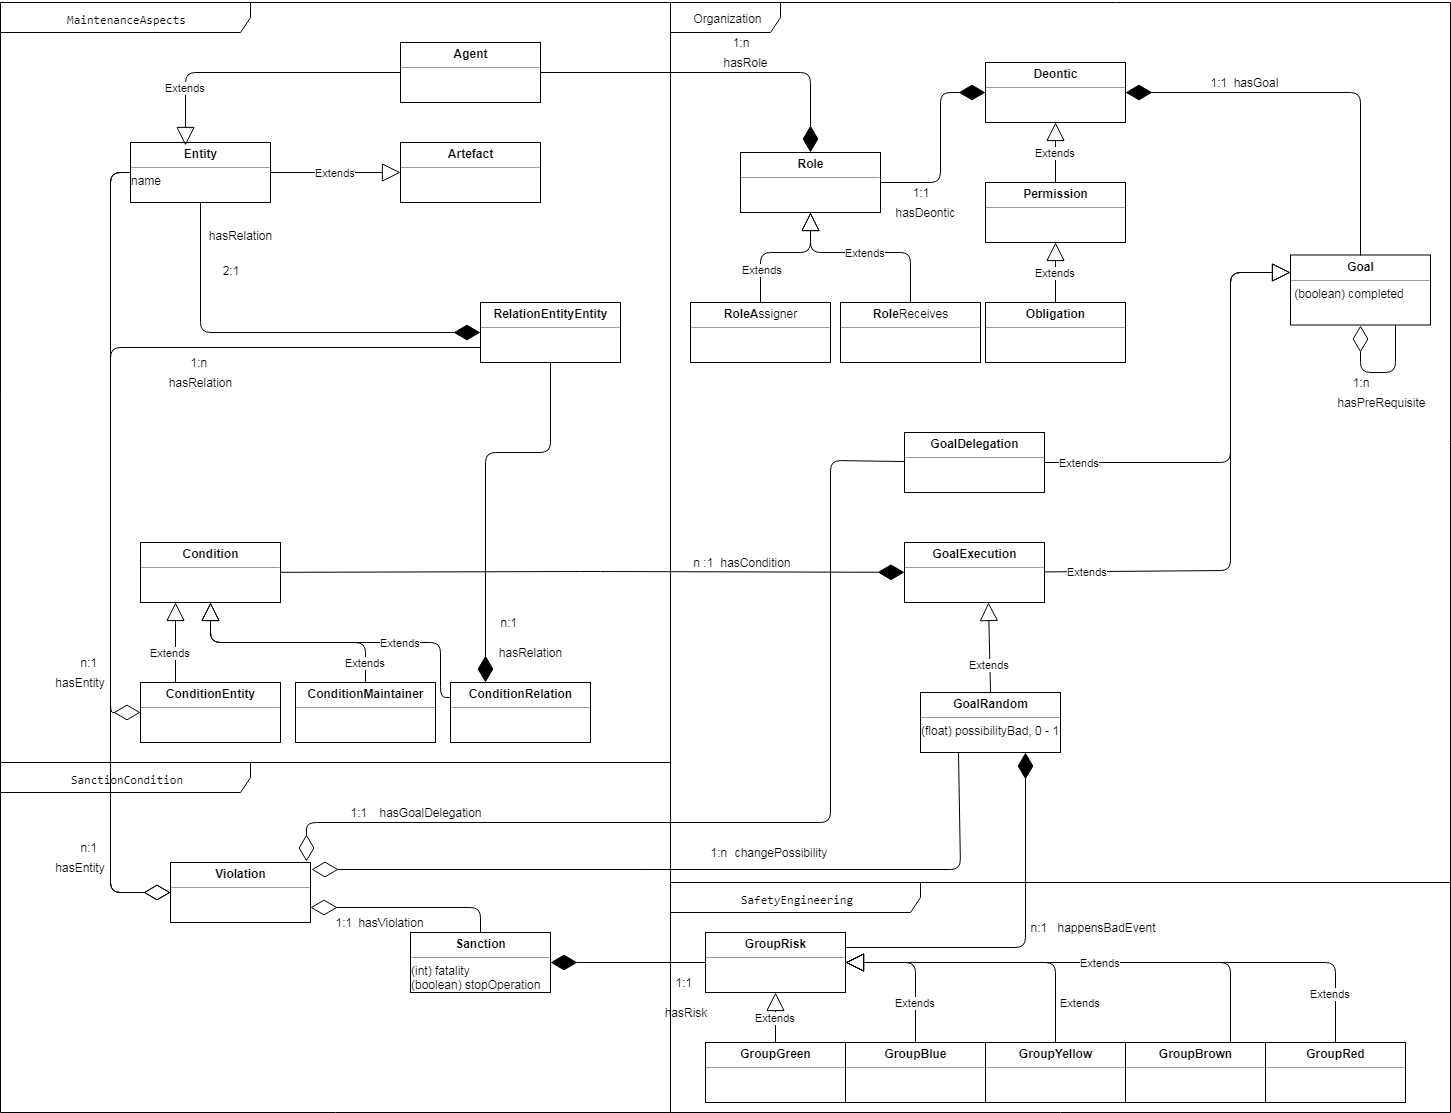
\includegraphics[width=0.8\linewidth]{umlmodel} 
\end{figure}


\bibliographystyle{sbc}
\bibliography{sbc-template}
\end{document} 
